%%%%%%%%%%%%%%%%%%%%%%%%%%%%%%%%%%%%%%%%%%%%%%%%%%%%%%%%%%%%%%%%%%%%%%%%%%%%%%%%
%                                                                              %
% decay_channels_1                                                             %
%                                                                              %
% version: 2016-03-21T1109Z                                                    %
%                                                                              %
% Will Breaden Madden                                                          %
%                                                                              %
%%%%%%%%%%%%%%%%%%%%%%%%%%%%%%%%%%%%%%%%%%%%%%%%%%%%%%%%%%%%%%%%%%%%%%%%%%%%%%%%
%                                                                              %
% DESCRIPTION                                                                  %
%                                                                              %
% This program produces a particle decay channels diagram.                     %
%                                                                              %
%%%%%%%%%%%%%%%%%%%%%%%%%%%%%%%%%%%%%%%%%%%%%%%%%%%%%%%%%%%%%%%%%%%%%%%%%%%%%%%%
%                                                                              %
% LICENCE INFORMATION                                                          %
%                                                                              %
% This program produces a document.                                            %
%                                                                              %
% copyright (C) 2016 William Breaden Madden                                    %
%                                                                              %
% This software is released under the terms of the GNU General Public License  %
% version 3 (GPLv3).                                                           %
%                                                                              %
% This program is free software: you can redistribute it and/or modify it      %
% under the terms of the GNU General Public License as published by the Free   %
% Software Foundation, either version 3 of the License, or (at your option)    %
% any later version.                                                           %
%                                                                              %
% This program is distributed in the hope that it will be useful, but WITHOUT  %
% ANY WARRANTY; without even the implied warranty of MERCHANTABILITY or        %
% FITNESS FOR A PARTICULAR PURPOSE.  See the GNU General Public License for    %
% more details.                                                                %
%                                                                              %
% For a copy of the GNU General Public License, see                            %
% <http://www.gnu.org/licenses/>.                                              %
%                                                                              %
%%%%%%%%%%%%%%%%%%%%%%%%%%%%%%%%%%%%%%%%%%%%%%%%%%%%%%%%%%%%%%%%%%%%%%%%%%%%%%%%

\documentclass[tikz]{standalone}
\usetikzlibrary{matrix}

\begin{document}

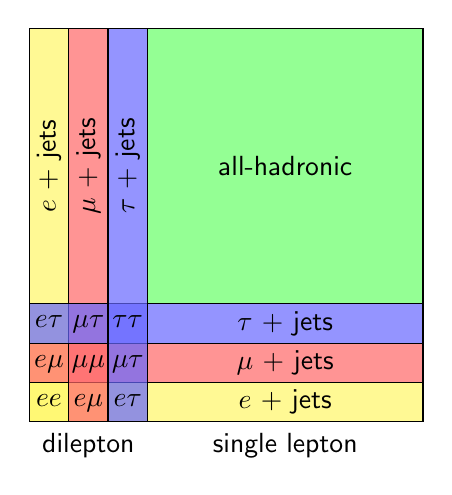
\begin{tikzpicture}[font=\sffamily]

\foreach\x[count=\xi from 0] in {yellow, red, blue}{
    \draw[fill=\x!60, fill opacity=0.7] (0, \xi * 5mm) rectangle (5, {(\xi + 1) * 5mm});
    \draw[fill=\x!60, fill opacity=0.7] (\xi * 5mm, 0) rectangle ({(\xi + 1) * 5mm}, 5);
}
\draw[fill=green!60, fill opacity=0.7] (1.5, 3 * 5mm) rectangle (5, {(9 + 1) * 5mm});
\matrix[
    matrix of math nodes,
    inner sep=0,
    outer sep=0,
    anchor=south west,
    nodes={
        anchor=center,
        text=black,
        minimum size=5mm,
        inner sep=0,
        outer sep=0,
        text height=1ex,
        text depth=0.25ex
    }
] at (0, 0){
    e\tau&\mu\tau&\tau\tau\\
    e\mu&\mu\mu&\mu\tau\\
    ee&e\mu&e\tau\\
};
\node[rotate=0] at (0.75, -0.3) {dilepton};
\node[rotate=0] at (3.25, -0.3) {single lepton};
\node[rotate=0] at (3.25, 1.25) {${\tau}$ + jets};
\node[rotate=0] at (3.25, 0.75) {${\mu}$ + jets};
\node[rotate=0] at (3.25, 0.25) {${e}$ + jets};
\node[rotate=90] at (0.25, 3.25) {${e}$ + jets};
\node[rotate=90] at (0.75, 3.25) {${\mu}$ + jets};
\node[rotate=90] at (1.25, 3.25) {${\tau}$ + jets};
\node[rotate=0] at (3.25, 3.25) {all-hadronic};

\end{tikzpicture}

\end{document}
